\section{Replication and fault tolerance}

Kafka was build with fault tolerance in mind. To achieve this Kafka uses replication. Replication involves storing identical copies of topics on multiple brokers. If we say that a topic has a replication factor of 3, this means 3 brokers have the exact same copy of the topic. For each topic a leader is elected. Producers and consumers only interact with the leader, then the data is replicated on followers. again if the replication factor is 3 then the leader will get the first copy and 2 more followers will copy the data from the leader. This is shown in figure \ref{fig:replication-leader}

\begin{figure}[H]
  \centering
  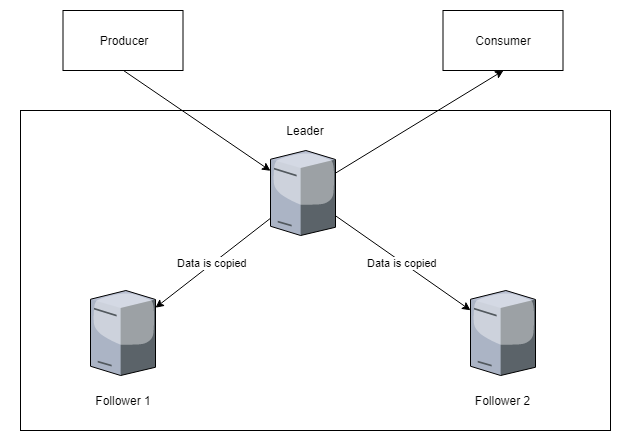
\includegraphics[scale=0.5,width=100mm]{./images/replication-leader.png}
  \caption{Producers and consumers only interact with the replication leader. Followers replicate the topic data}
  \label{fig:replication-leader}
\end{figure}

When a broker goes down, we will still be able to serve the topic data as it has been replicated on multiple brokers. When a leader goes down, an election is held. One important point is that every write from the producer through the leader gets assigned a special id called a zxid. A zxid is assigned only if the majority of followers have sent an ACK to the leader. If the leader goes down, each follower will attempt to become the new leader by broadcasting the last zxid that they have. The other followers will reply with an OK message if the zxid is less than the last one they have seen. If they others have one that is higher than the broadcasted zxid then they will send a NO response. The leader will be elected by the follower who has the majority of OK responses. 